%Copyright 2014 Jean-Philippe Eisenbarth
%This program is free software: you can
%redistribute it and/or modify it under the terms of the GNU General Public
%License as published by the Free Software Foundation, either version 3 of the
%License, or (at your option) any later version.
%This program is distributed in the hope that it will be useful,but WITHOUT ANY
%WARRANTY; without even the implied warranty of MERCHANTABILITY or FITNESS FOR A
%PARTICULAR PURPOSE. See the GNU General Public License for more details.
%You should have received a copy of the GNU General Public License along with
%this program.  If not, see <http://www.gnu.org/licenses/>.

%Based on the code of Yiannis Lazarides
%http://tex.stackexchange.com/questions/42602/software-requirements-specification-with-latex
%http://tex.stackexchange.com/users/963/yiannis-lazarides
%Also based on the template of Karl E. Wiegers
%http://www.se.rit.edu/~emad/teaching/slides/srs_template_sep14.pdf
%http://karlwiegers.com
\documentclass{scrreprt}
\usepackage{listings}
\usepackage{underscore}
\usepackage[bookmarks=true]{hyperref}
\usepackage[utf8]{inputenc}
\usepackage[english]{babel}
\usepackage{longtable}
\usepackage{graphicx}
\graphicspath{ {./images/} }
\hypersetup{
    colorlinks=true,
    bookmarks=false,    % show bookmarks bar?
    pdftitle={Design Document},    % title
    pdfauthor={Jean-Philippe Eisenbarth},                     % author
    pdfsubject={TeX and LaTeX},                        % subject of the document
    pdfkeywords={TeX, LaTeX, graphics, images}, % list of keywords
    colorlinks=true,       % false: boxed links; true: colored links
    linkcolor=blue,       % color of internal links
    citecolor=black,       % color of links to bibliography
    filecolor=black,        % color of file links
    urlcolor=purple,        % color of external links
    linktoc=page            % only page is linked
}%
\def\myversion{1.0 }
\date{}
%\title
\usepackage{hyperref}
\begin{document}

\begin{flushright}
    \rule{16cm}{5pt}\vskip1cm
    \begin{bfseries}
        \Huge{SOFTWARE ARCHITECTURE}\\
        \vspace{1.9cm}
        for\\
        \vspace{1.9cm}
        GBUS Scheduling App\\
        \vspace{1.9cm}
        \LARGE{Version \myversion approved}\\
        \vspace{1.9cm}
        Prepared by Jack Doiron, Jared Cassarly, Shota Nemoto, Martin Peters\\
        \vspace{1.9cm}
        \today\\
    \end{bfseries}
\end{flushright}

\tableofcontents


\chapter*{Revision History}

\begin{center}
    \begin{tabular}{|c|c|c|c|}
        \hline
	    Name & Date & Reason For Changes & Version\\
        \hline
	    Jack Doiron & 2/22/19 & initial draft & 1.0 draft 1\\
        \hline
    \end{tabular}
\end{center}

\chapter{Introduction}

\section{References}
UIPatterns.io. \textit{UI Patterns},\\
http://uipatterns.io

\chapter{User Interface}

This section explains the design for the requirements mentioned in section 3.1 of the Software Requirements Specification document.

\section{Home Screen}

The Home Screen will be the default page for the application.  It will display the current date, Toolbar, and a view of the user's calendar of events if logged in.  If the user is not logged in, the calendar will be empty. See Figure 2a-2c for a skeleton of the Home Screen on each view mode.\\
\\
When the application opens, the calendar will show the view with the current day.  swiping left or right will allow the user to look at future or past events (respectively) based on the currently selected view mode.\\
\\
The Home Screen will also have a Hamburger Menu where the user can access their account information and the General Settings.\\
\\
In regards to account information, the user will be able to bring up fields to change their account email and password.  Additionally, the user will be able to bring up login, logout, and registration menus from the Hamburger Menu.  See Figure 3a for a skeleton of the Hamburger Menu when the user is logged in and Figure 3b for a skeleton of the Hamburger Menu when the user is logged out.\\
\\
Finally, the Home Screen will need to load in less than 3 seconds. \\
\\
\\
Below is the activity diagram of a typical user's actions from the home screen:\\
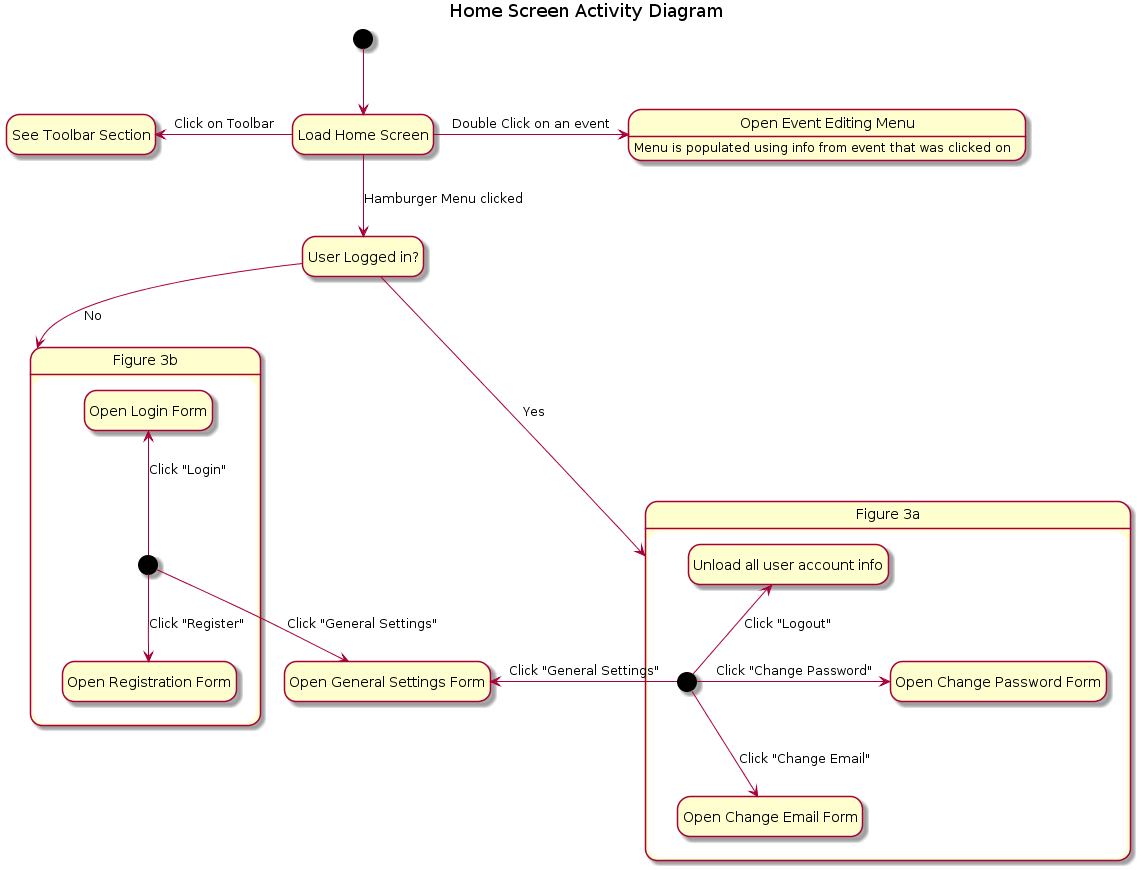
\includegraphics[width=\textwidth]{./images/homescreen.png}

\subsection{Attributes}

\begin{center}
\begin{longtable}{ | p{5cm} | p{5cm} | p{5cm} | }
\hline
\textbf{Attribute Name} & \textbf{Type} & \textbf{Description} \\
\hline
events & Event[] & The list of events being displayed on the calendar \\
\hline
toolbarState & Toolbar & The object that stores the state of the Toolbar for the calendar \\
\hline
date & Date Object & the date being displayed on the Home Screen
\hline
hamburgerMenuState & Boolean & true if the Hamburger Menu is open, false if closed \\
\hline
selectedTool & ToolEnum & Enermerated value that indicates which tool is currently selected. Used to determine behavior when user clicks on schedule. Values include: CUT, COPY, PASTE, DRAGDROP, 
RESIZE.\\
\hline
diffViewState & DiffView & The object that stores the state of the Auto Scheduler Diff View for newly generated schedules.\\
\hline
\end{longtable}
\end{center}

\subsection{Methods}

\begin{center}
\begin{longtable}{ | p{5cm} | p{2cm} | p{3cm} | p{5cm} | }
\hline
\textbf{Method Name} & \textbf{Return Type} & \textbf{Parameters} & \textbf{Description} \\
\hline
displayEvents & void & void & Syncs from the server and displays the received events appropriately on the calendar based on the view mode and Figure 2 \\
\hline
displayToolbar & void & void & Displays all the parts of the Toolbar defined below as per Figure 2 \\
\hline
displayDate & void & void & Displays the date at the top of the screen as per Figure 2 \\
\hline
displayHamburgerMenu & void & void & Displays the Hamburger Menu in the top right of the screen as per Figure 2 \\
\hline
toolbarEventListener & void & void & Listens for events from the toolbar and updates the GUI accordingly \\
\hline
openHamburgerMenu & void & void & Opens the Hamburger Menu overlay when the user clicks the button \\
\hline
closeHamburgerMenu & void & void & Closes the Hamburger Menu overlay when the user clicks off the menu when it is open \\
\hline
hamburgerEventListener & void & void & Waits for the user to click on a button in the Hamburger Menu and then performs the relevant function. \\
\hline
userClick & void & UIEvent & Responds to user clicks on schedule. Behavior depends on currently selected tool as described in Toolbar section below.\\
\hline
\end{longtable}
\end{center}

The first 4 methods that display items on the Home Screen are called whenever the user moves to the Home Screen.

\section{Abstract Input Form}

Whenever the application needs to get data based on Figure 1, the UI class will have the following methods:

\subsection{Attributes}

\begin{center}
\begin{longtable}{ | p{3cm} | p{3cm} | p{9cm} | }
\hline
\textbf{Attribute Name} & \textbf{Type} & \textbf{Description} \\
\hline
FieldEnum & Final Enum & Enum object that specifies the choices for the type of input field to load: STANDARD, LOCATION, DEADLINE, SETTINGS, and EVENT.  EVENT specifies a drop-down menu to load for choosing a different enum value. \\
\hline
\end{longtable}
\end{center}

\subsection{Methods}

\begin{center}
\begin{longtable}{ | p{3cm} | p{2cm} | p{2cm} | p{8cm} | }
\hline
\textbf{Method Name} & \textbf{Return Type} & \textbf{Parameters} & \textbf{Description} \\
\hline
loadInputFields & abstract void & FieldEnum & Loads the proper input fields based on the Event type specified by the FieldEnum passed in.\\
\hline
waitForUserInput & void & void & Waits for the user to fill out the form and click back or save. \\
\hline
saveForm & abstract void & void & Saves the changes the user made and handles the storage appropriately \\
\hline
back & void & void & Checks if there are unsaved changes to the fields in the form being edited.  If there are unsaved changes, it displays a pop-up that asks the user if they really want to exit the form.  If they do, then it discards the changes and calls exitForm.  Otherwise, the application continues waiting for user input on the form.  If there are no unsaved changes, then the application just calls exitForm.\\
\hline
exitForm & void & void & Leaves the form and goes back to the Home Screen \\
\hline
\end{longtable}
\end{center}

This form should load in less than 3 seconds. \\

\section{Event Editing and Creation Menu}

When the user wants to create an event, they will be able to click the Create event on the Toolbar.  When they do so, they will be presented with a choice of creating a Standard, Location, or Deadline event (from a drop down menu). Once the user makes their decision, a form with the necessary items to create an event will be displayed.  All of the items will have default values filled in based on the General Settings or global defaults.
\\\\
Additionally, the same form can be pulled up from any existing event by clicking on  it.  All the default values in the form will be the values stored in the chosen Event object.
\\\\
The form the user sees will have a skeleton matching figure 1 where each field follows the format specified by \textit{UI Patterns}.  Thus, the event editing/creation menu will extend the Abstract Input Form Class.
\\\\
Once the user finishes filling in the form, they can either save the form and go back to the Home Screen or discard the changes and return to the Home Screen.
\\
One exception to the aforementioned exiting process is with Deadline events.  Once the user clicks save on a Deadline event, they will be presented with a diff between their old calendar and the changes the auto scheduler proposes based on the information provided for the deadline event.  The user will be given the option to accept the changes or reject them (returning them to the input form).  Upon acceptance, the changes are saved and the user goes back to the home screen.
\\\\
The following diagram shows the flow of this editing/creation process.
\\\\
\begin{center}
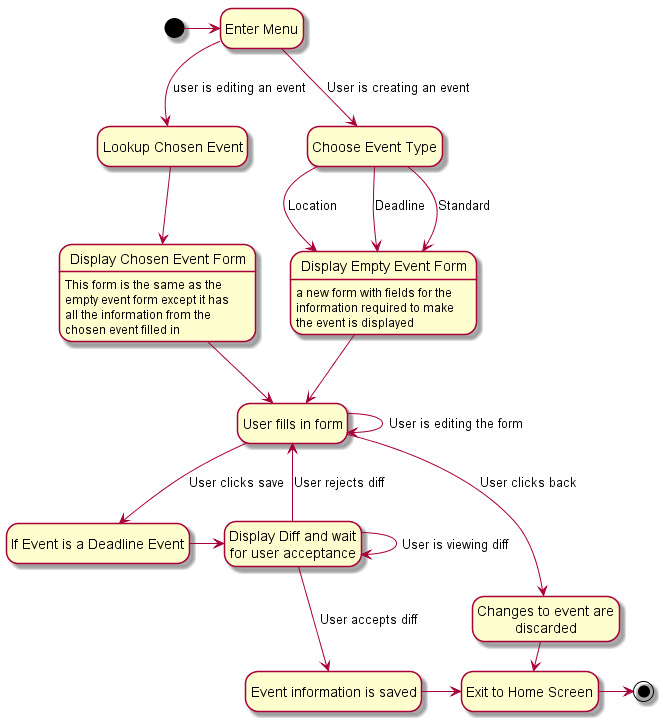
\includegraphics[scale=0.5]{edit.png}
\end{center}

\subsection{Standard Event Input Fields}
The following table describes the input fields shown to the user for a Standard Event
\begin{center}
\begin{longtable}{ | p{3cm} | p{8cm} | p{4cm} | }
\hline
\textbf{Field Name} & \textbf{Field Type} & \textbf{Default Value for Creation} \\
\hline
Name & Text Field & "" \\
\hline
Description & Text Field & "" \\
\hline
Event Start & Time and Date Input & Current Time and Date \\
\hline
Event End & Time and Date Input & Current Time and Date \\
& & Plus General Settings \\
& & Default Duration \\
\hline
Location & Text Field with Suggestions & General Settings \\
& based on other event locations & Default \\
\hline
Frequency & Drop Down with following choices & Just Once \\
& - Just Once & \\
& - Daily & \\
& - Weekly & \\
& - Monthly & \\
& - Yearly & \\
& - Custom & \\
\hline
Notifications & Drop Down with following choices & General Settings\\
& - Email & Default\\
& - Text & \\
& - Banner & \\
& - Push & \\
& - None & \\
\hline
Notification Time & Number (in minutes) & General Settings \\
Before Event & & Default \\
\hline
Locked & Checkbox & True \\
\hline
\end{longtable}
\end{center}

The custom option for frequency causes a popup like in Figure 4 to come up and the user then chooses the days of the week their event repeats on.  Once they do that, the custom settings are saved and then frequency field is completed and updated.

\subsection{Location Event Input Fields}
The Location event will have have the same input fields as the Standard event except without the Locked field

\subsection{Deadline Event Input Fields}
The following table describes the input fields shown to the user for a Deadline Event

\begin{center}
\begin{longtable}{ | p{3cm} | p{8cm} | p{4cm} | }
\hline
\textbf{Field Name} & \textbf{Field Type} & \textbf{Default Value for Creation} \\
\hline
Name & Text Field & "" \\
\hline
Description & Text Field & "" \\
\hline
Task Start Time & Time and Date Input & Current Time and Date \\
\hline
Task Deadline & Time and Date Input & Current Time and Date \\
& & Plus General Settings \\
& & Default Duration \\
\hline
Location & Text Field with Suggestions & General Settings \\
& based on other event locations & Default \\
\hline
Use Location & Checkbox & True \\
For Auto & & \\
Scheduling & & \\
\hline
Minimum Time & Number & General Settings \\
for Scheduled & & Default\\
Events & & \\
\hline
Maximum Time & Number & General Settings \\
for Scheduled & & Default\\
Events & & \\
\hline
Minimum Break & Number & General Settings \\
Time between & & Default\\
 Scheduled Events & & \\
\hline
Total Time to & Number (in Hours) & Task Deadline \\
Complete Task & & - Task Start Time \\
\hline
\end{longtable}
\end{center}

\subsection{Attributes}

The event editing and creation menu will have all attributes from the parent Abstract Input Form class along with the following:

\begin{center}
\begin{longtable}{ | p{3cm} | p{3cm} | p{9cm} | }
\hline
\textbf{Attribute Name} & \textbf{Type} & \textbf{Description} \\
\hline
accountEvents & Event[] & Reference to the list of events on the user's account \\
\hline
\end{longtable}
\end{center}

Additionally, the edit/creation form will not use the SETTINGS field in the FieldEnum.

\subsection{Methods}

The event editing and creation menu will have all methods from the parent Abstract Input Form class along with the following:

\begin{center}
\begin{longtable}{ | p{3cm} | p{1cm} | p{2cm} | p{9cm} | }
\hline
\textbf{Method Name} & \textbf{Return Type} & \textbf{Parameters} & \textbf{Description} \\
\hline
loadInputFields & void & FieldEnum & Loads the proper input fields based on the Input Field type specifed by the FieldEnum passed in. STANDARD, LOCATION, and DEADLINE specify the corresponding input fields from above.  DEFAULT specifies that a drop-down menu to get ask for a different FieldEnum should be used. \\
\hline
saveForm & void & void & Saves the changes the user made and adds the event to the account's Event list
\hline
displayDiff & void & void & Displays the auto-scheduler diff for Deadline Events when the user finishes filling out the form. Also waits for the user to accept or reject the diff. \\
\hline
\end{longtable}
\end{center}

Note that the loadInputFields method is called with the DEFAULT input when a event is being created. Once the user selects and event type, the same method is called again based on the chosen event type.\\\\
If the user us editing an event, loadInputFields gets the event type based on teh type of event being edited.\\\\

\section{General Settings Menu}

The General Settings Menu will be accessible from the Hamburger Menu on the home screen.  When the user enters the General Settings Menu, the application will look up the settings and load them into a series of input fields they they can edit.  When the user saves their changes to the form, they will return to the Home Screen.  If the user clicks the back button without saving, they will be prompted with a pop-up that checks to make sure they really want to leave without saving.  If they say yes, their changes will not be saved and they will go back to the Home Screen.  Otherwise, they will not leave the General Settings and can continue editing.
\\\\
The following state diagram depicts the above process:
\\\\
\begin{center}
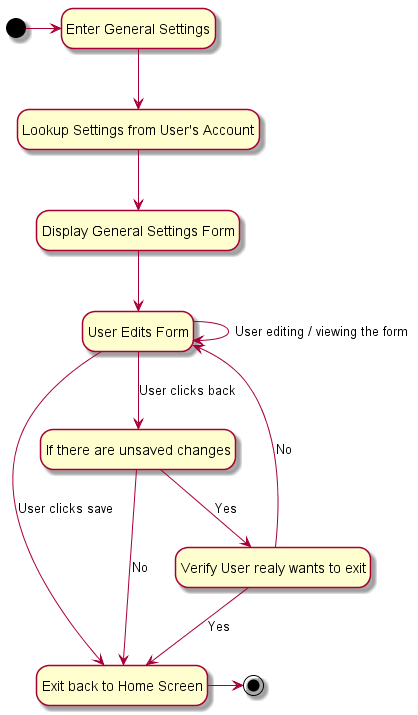
\includegraphics[scale=0.5]{settings.png}
\end{center}
The UI will utilize the skeleton depicted in Figure 1 where each field follows the format specified by \textit{UI Patterns}.
\\\\
The information on this page will include all items specified in the General Settings Requirements.  The following table describes the Input Fields in more detail:

\subsection{Input Fields}

\begin{center}
\begin{longtable}{ | p{3cm} | p{6cm} | p{6cm} | }
\hline
\textbf{Field Name} & \textbf{Field Type} & \textbf{Default from Requirements} \\
\hline
Snap to Grid & Number (in minutes) & Settings.Toolbar.SnapToGrid.Default \\
\hline
Auto Scheduler & Number (in minutes) & Settings.AutoScheduling. \\
Break Time & & MinOpenTime.Default\\
\hline
Auto Scheduler & Number (in minutes) & Settings.AutoScheduling. \\
Min Event Time & & MinTime.Default\\
\hline
Auto Scheduler & Number (in minutes) & Settings.AutoScheduling. \\
Max Event Time & & MaxTime.Default\\
\hline
Language & Drop Down Menu with all & Settings.Language.Default \\
& supported languages as options & \\
\hline
Notifications & Drop Down with following choices & Settings.Events.Notifications.Default \\
& - Email & Default\\
& - Text & \\
& - Banner & \\
& - Push & \\
& - None & \\
\hline
Notification Time & Number (in minutes) & Settings.Events.Notifications. \\
Before Event & & Time.Default \\
\hline
Event Duration & Number (in minutes) & Settings.Events.Duration.Default \\
\hline
Location & Text Field with Suggestions & Settings.Events.Location.Default \\
& based on other event locations & \\
\hline
\end{longtable}
\end{center}
The constraints specified in the Settings.AutoScheduling.* Requirements will be checked while the user is entering the form and if the constraints are not met, the user will be unable to save their changes.
\\\\
Note that the Settings.AutoScheduling.MinOpenTime Requirement was merged with the Settings.AutoScheduling.Breaks Requirement since they represent the same thing.
\\\\
The general settings menu will extend the Abstract Input Form Class

\subsection{Attributes}

The general settings menu will have all attributes from the parent Abstract Input Form class along with the following:

\begin{center}
\begin{longtable}{ | p{3cm} | p{3cm} | p{9cm} | }
\hline
\textbf{Attribute Name} & \textbf{Type} & \textbf{Description} \\
\hline
accountSettings & Settings[] & Reference to the list of settings on the user's account \\
\hline
\end{longtable}
\end{center}

\subsection{Methods}

The general settings menu will have all methods from the parent Abstract Input Form class along with the following:

\begin{center}
\begin{longtable}{ | p{3cm} | p{2cm} | p{2cm} | p{8cm} | }
\hline
\textbf{Method Name} & \textbf{Return Type} & \textbf{Parameters} & \textbf{Description} \\
\hline
loadInputFields & void & FeildEnum & Loads the input fields specified in the General Settings Input Field table above. Should always receive the SETTINGS value as the parameter.\\
\hline
saveForm & void & void & Saves the changes the user made and adds the event to the account's settings \\
\hline
\end{longtable}
\end{center}

\section{Account Management}

The user can sign up for an account, login, logout, or reset their password.  The Sign Up UI should come up upon opening the app while not logged in and after signing out.

Each form sends a post request to the relevant part of the server.

\subsection{Account Management Form Fields}
\begin{center}
\begin{longtable}{ | p{3cm} | p{4cm} | p{8cm} | }
\hline
\textbf{Field Name} & \textbf{Field Type} & \textbf{Description} \\
\hline
email & Text Field & the user's email address \\
\hline
password & Password Field & password of the user \\
\hline
second password & Password Field & second password field to verify the user's password\\
\hline
\end{longtable}
\end{center}

\subsection{Account Management Interfaces}
There are 3 user interfaces related to account management:\\
\textbf{Log In:}
logs the user in.  Uses the email and password fields.
\begin{center}
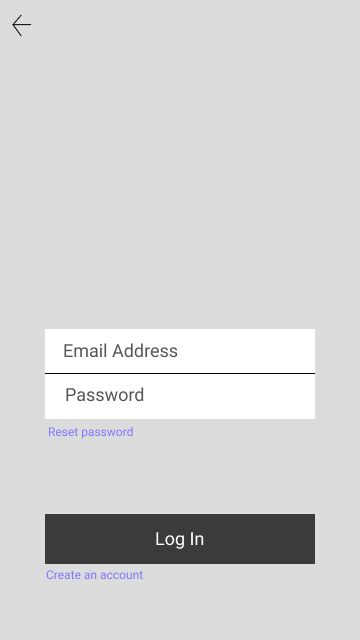
\includegraphics[scale=0.4]{login.png}
\end{center}

\textbf{Reset Password:}
Tells the server to send a reset password email.  Uses email field.
\begin{center}
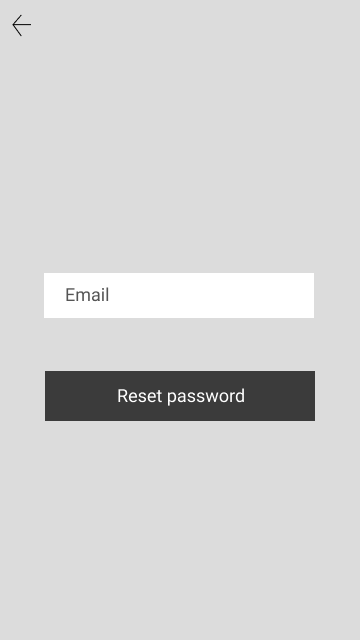
\includegraphics[scale=0.4]{resetpass.png}
\end{center}

\textbf{Sign Up:}
Requests the server to sign the user up.  Uses the email, password, and second password fields.
\begin{center}
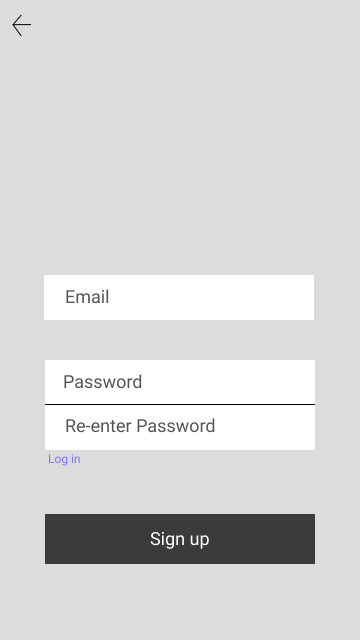
\includegraphics[scale=0.4]{signup.png}
\end{center}

\section{Auto Scheduler Diff View}
The Auto Scheduler Diff view allows the user to view both the old calendar with all existing events in their original state and the new calendar with new events created for the user's deadlines along with updated times for unlocked events.\\
This view opens and replaces the normal schedule in the home screen whenever the Auto Scheduler generates a new schedule.

\subsection{Attributes}
\begin{center}
\begin{longtable}{ | p{3cm} | p{3cm} | p{9cm} | }
\hline
\textbf{Attribute Name} & \textbf{Type} & \textbf{Description} \\
\hline
OriginalEvents & Event[] & Original list of events on the user's calendar.\\
\hline
NewEvents & Event[] & New list of events generated by Auto Scheduler.\\
\hline
AcceptButton & Button & Button that accepts the new schedule when pressed.\\
\hline
DeclineButton & Button & Button that declines the new schedule when pressed.\\
\hline
\end{longtable}
\end{center}

\subsection{Methods}
\begin{center}
\begin{longtable}{ | p{3cm} | p{2cm} | p{2cm} | p{9cm} | }
\hline
\textbf{Method Name} & \textbf{Return Type} & \textbf{Parameters} & \textbf{Description} \\
\hline
show & void & void & Makes the Auto Scheduler Diff View visible.\\
\hline
close & void & vod & Closes the Auto Scheduler Diff View. Does not save changes to user's schedule\\
\hline
setOriginalSchedule & void & Event[] & Sets the list containing events on the user's original schedule.\\
\hline
setNewSchedule & void & Event[] & Sets the list containing events from Auto Scheduler's schedule.\\
\hline
accept & void & void & Closes the Auto Scheduler Diff View and saves changes made to the user's schedule.\\
\hline
\end{longtable}
\end{center}

\begin{center}
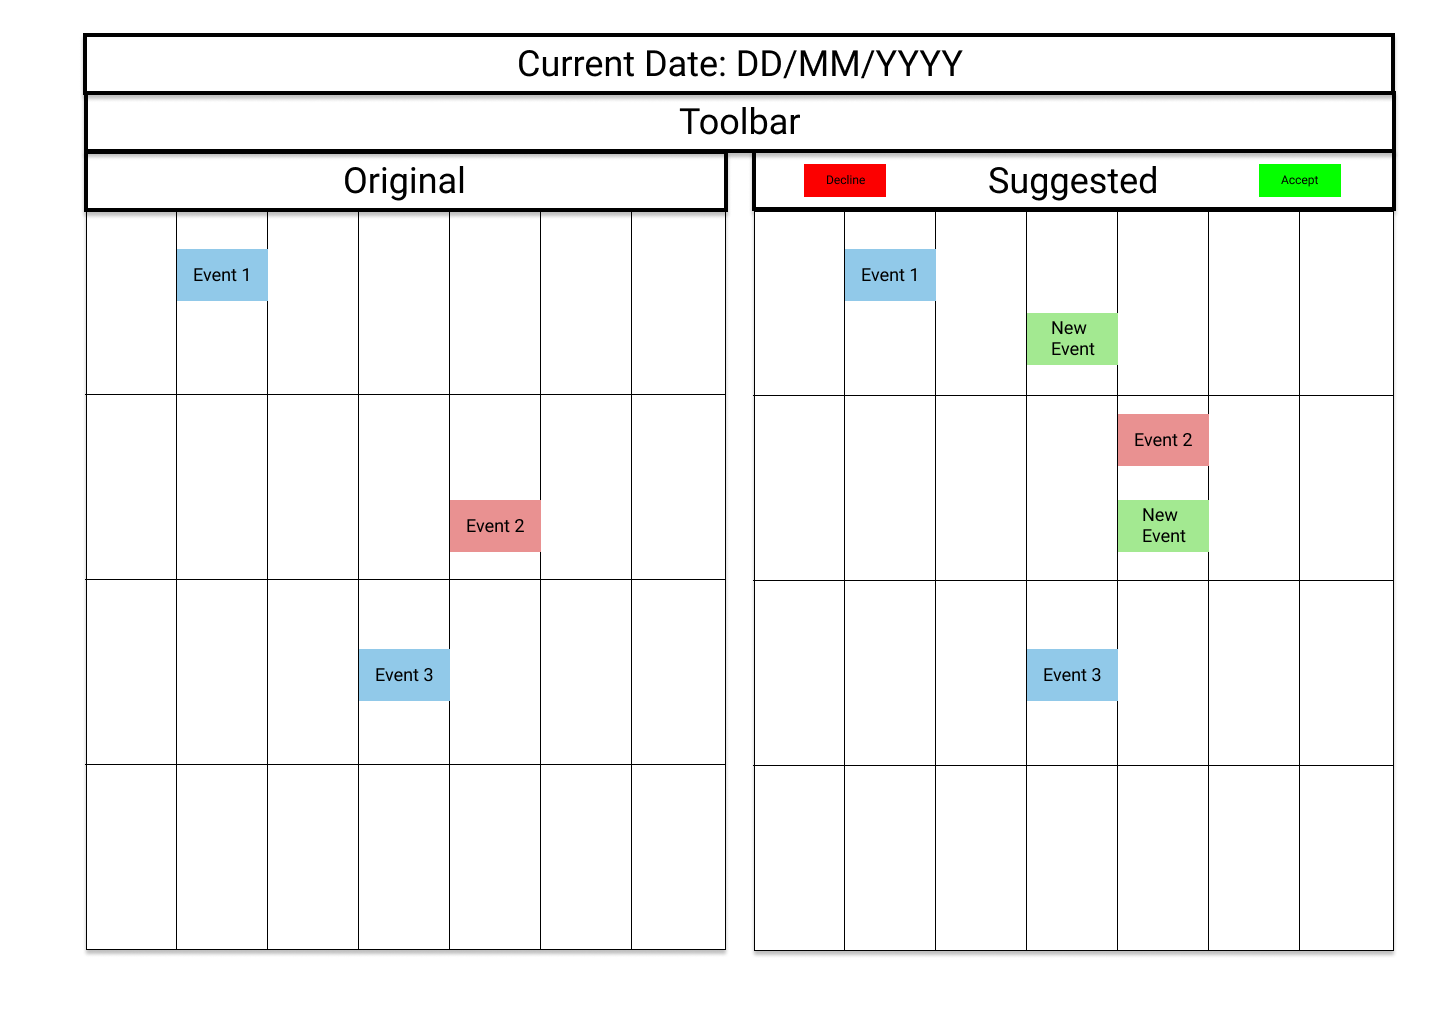
\includegraphics[width=\textwidth]{diff.png}
\end{center}

\section{Toolbar}

\subsection{Description}
The toolbar will allow the user to edit their schedule in the application's graphical display.
Each individual tool can be selected by clicking on the tool's corresponding icon, and deselected by clicking on the icon again. The tools provided on the toolbar will be: drag and drop, re-size, cut, copy, paste. Additionally, there will be buttons on the toolbar to create and event, edit an event, and change the view mode of the schedule.
The tools' behaviors will be handled within the Home Screen's userClick() method.

\subsection{Attributes}
\begin{center}
\begin{longtable}{ | p{3cm} | p{3cm} | p{9cm} | }
\hline
\textbf{Attribute Name} & \textbf{Type} & \textbf{Description} \\
\hline
SelectedTool & ToolEnum & Enermerated value that indicates which tool is currently selected on the toolbar. Values include CUT, COPY, PASTE, DRAGDROP, and RESIZE.\\
\hline
DragDropButton & Button & A button with the drag and drop tool icon on it. Changes SelectedTool to DragDrop.\\
\hline
ResizeButton & Button & A button with the re-size tool icon on it. Changes SelectedTool to Resize.\\
\hline
CutButton & Button & A button with the cut tool icon on it. Changes SelectedTool to Cut.\\
\hline
CopyButton & Button & A button with the copy tool icon on it. Changes SelectedTool to Copy.\\
\hline
PasteButton & Button & A button with the paste tool icon on it. Changes SelectedTool to Paste.\\
\hline
CreateButton & Button & A button labelled "Create". Opens event creation form.\\
\hline
ViewButton & Button & A button labelled "View". Cycles through view modes.\\
\hline
\end{longtable}
\end{center}

\subsection{Interface Methods}
\begin{center}
The toolbar object will be part of the Home Screen page, stored in the toolbarState attribute. Its interface consists of the following methods of notifying the Home Screen of events that occur within the toolbar.
\begin{longtable}{ | p{3cm} | p{2cm} | p{2cm} | p{9cm} | }
\hline
\textbf{Method Name} & \textbf{Return Type} & \textbf{Parameters} & \textbf{Description} \\
\hline
listen & void & void & Toolbar waits for user to click a button on the toolbar.\\
\hline
currentTool & enum & void & Toolbar indicates which tool is currently selected on it.\\
\hline
notifyUIEvent & UIEvent & void & This function is called internally to notify any objects subscribed to the toolbar of an event that occurred. This will generally be used when the user clicks on a button.\\
\hline
\end{longtable}
\end{center}

\subsection{Drag and Drop Events}
This tool will be used to move the start and end times of an event from the graphical user interface (GUI) (Requirement: Toolbar.DragDrop). This tool will generally follow this sequence of events:
\begin{enumerate}
    \item User clicks on drag and drop icon in the toolbar. (requirement: Toolbar.Select.DragDrop)\\
    \\ & The GUI's event listener now responds to user clicks on events with only the drag and drop tool. An attribute in the GUI will be an enumerated value and be set to a value predefined as the drag and drop tool.
    \item User clicks anywhere within the event and does not release. Clicking the icon while the drag and drop tool is selected returns (requirement: Toolbar.DragDrop.Drag)\\
    \\ & The event will follow the user's cursor position with its top edge moved to the grid line closest to the user's cursor. The grid settings can be changed from the General Settings page.
    \item User releases event. (requirement: Toolbar.DragDrop.Release)\\
    \\ & The event's start time will be set to the time represented by the closest grid line when the user releases. The end time will be updated to maintain the original duration of the event.
\end{enumerate}
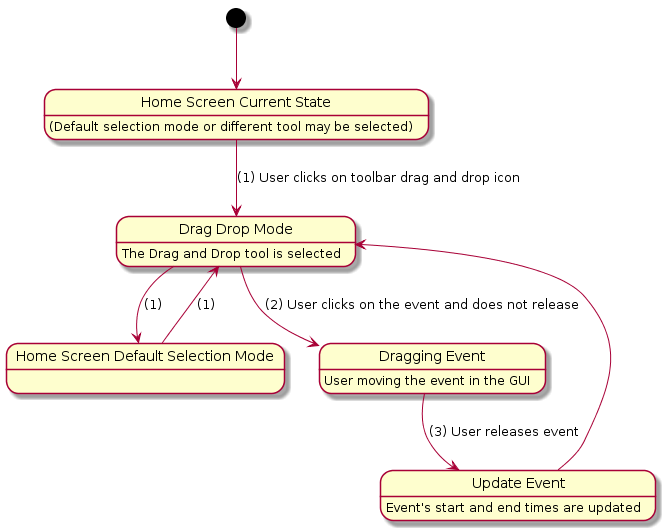
\includegraphics[width=\textwidth]{dragdrop.png}

\subsection{Resize Events}
This tool will be used to change the duration of an event from the GUI. This tool will generally follow this sequence of events:
\begin{enumerate}
    \item User clicks on re-size icon in the toolbar. (requirement: Toolbar.Select.Re-size)\\
    \\ & The GUI's event listener now responds to user clicks on events with only the re-size tool. An attribute in the GUI will be an enumerated value and be set to a value predefined as the re-size tool.
    \item User clicks on the top or bottom edge of an event and does not release. (requirement: Toolbar.Re-size.DragEdge)\\
    \\ & The selected edge of the event in the GUI will move up or down following the vertical movement of the user's cursor. The edge will move to the grid line closest to the user's cursor. The right and left edges of the event cannot be dragged.
    \item User releases edge. (requirement: Toolbar.Re-size.Release)\\
    \\ & If the user had clicked on the top edge of the event, the start time of the event will be updated to the time represented by the closest grid line when the user releases. Else, if the user had clicked on the bottom edge of the event, the end time of the event will be updated.
\end{enumerate}
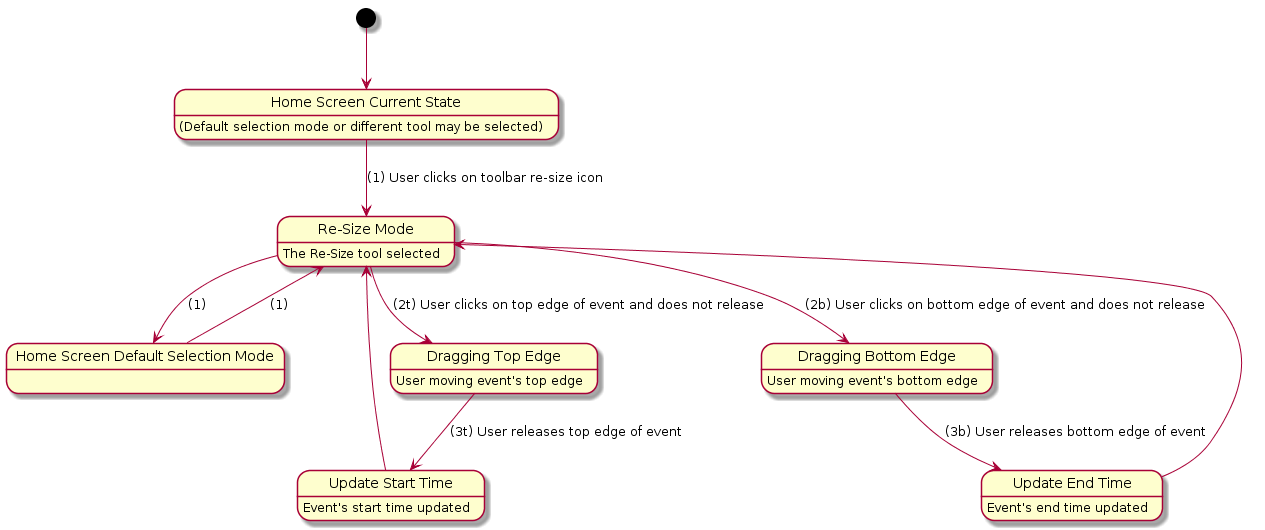
\includegraphics[width=\textwidth]{resize.png}

\subsection{Cut}
This tool will be used to save and remove an event from the schedule via the GUI. This tool will generally follow this sequence of events:
\begin{enumerate}
    \item User clicks on cut tool icon in the toolbar. (requirement: Toolbar.Select.Cut)\\
    \\ & The GUI's event listener now responds to user clicks on events with only the cut tool. An attribute in the GUI will be an enumerated value and be set to a value predefined as the copy tool.
    \item User clicks anywhere in the event and releases. (requirement: Toolbar.Cut)\\
    \\ & The event is removed from the GUI and the user's schedule. It is saved within the program for the creation of future copies of the event. The attributes that must be saved include its location, notification settings, locked status, description, name, duration, and parent if it is a deadline event. It replaces whatever previous event was stored in memory.
\end{enumerate}
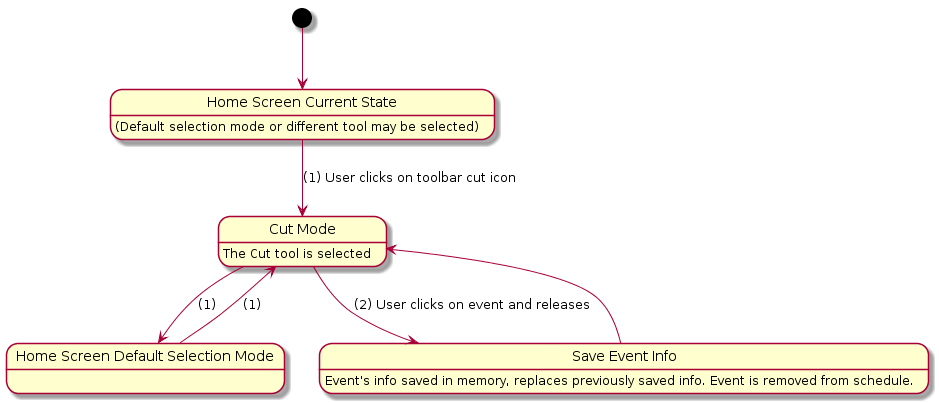
\includegraphics[width=\textwidth]{cut.png}

\subsection{Copy}
This tool will be used to save an event from the schedule via the GUI. Unlike the cut tool above, it will preserve the original event in the schedule. This tool will generally follow this sequence of events:
\begin{enumerate}
    \item User clicks on copy tool icon in the toolbar. (requirement: Toolbar.Select.Copy)\\
    \\ & The GUI's event listener now responds to user clicks on events with only the copy tool. An attribute in the GUI will be an enumerated value and be set to a value predefined as the copy tool.
    \item User clicks anywhere in the event and releases. (requirement: Toolbar.Copy)\\
    \\ & The event is saved within the program for the creation of future copies of the event. The attributes that must be saved include its location, notification settings, locked status, description, name, duration, and parent if it is a deadline event. It replaces whatever previous event was stored in memory. The original event remains in the schedule unchanged.
\end{enumerate}
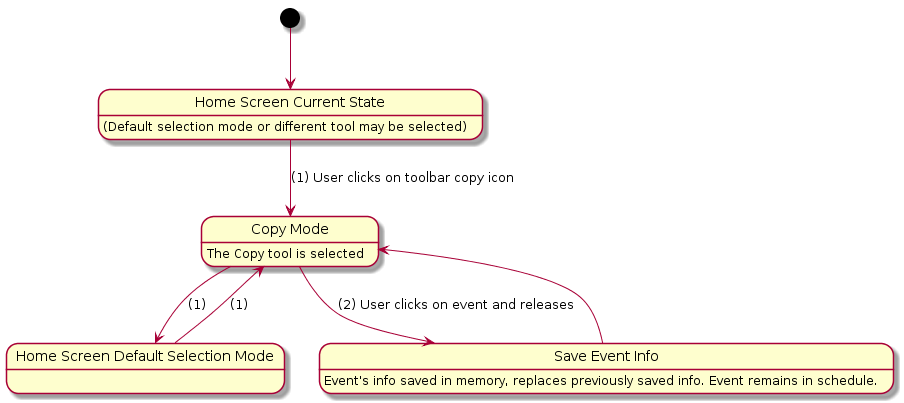
\includegraphics[width=\textwidth]{copy.png}

\subsection{Paste}
This tool will be used to create a new event using the data from an event previously saved using the cut or copy tool via the GUI. This tool will generally follow this sequence of events:
\begin{enumerate}
    \item User clicks on paste tool icon in the toolbar (requirement: Toolbar.Select.Paste)\\
    \\ & The GUI's event listener now responds to user clicks on the schedule with only the paste tool. An attribute in the GUI will be an enumerated value and be set to a value predefined as the paste tool.
    \item User clicks and releases anywhere on the schedule (requirement: Toolbar.Paste)\\
    \\ & A new event will be created in the GUI and in the user's schedule with the same location, notification settings, locked status, description, name, and parent if it is a deadline event, as the event saved in memory. The start time will be set to the time represented by the closest grid line and the end time will be set to the appropriate time following the new start time to maintain the original event's duration. If there is no event stored in memory, no new event will be created. Events created with this tool can overlap with existing events.
\end{enumerate}
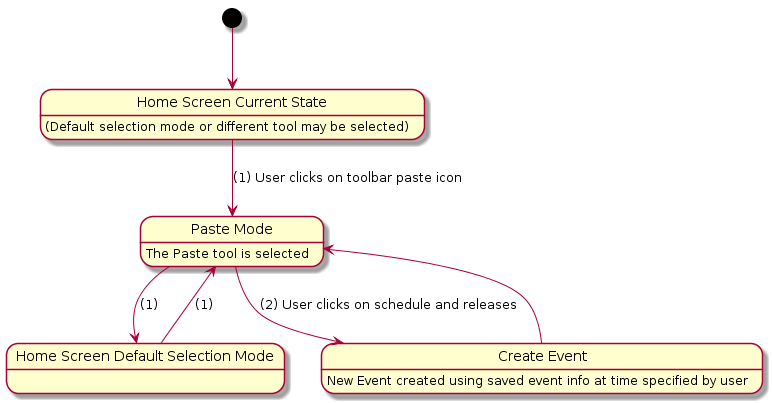
\includegraphics[width=\textwidth]{paste.png}

\subsection{View Mode}

The Toolbar's last item will allow the user to cycle through the method in which the calendar displays events.  There are 3 views that the user can choose from: Day, Week Month. \\
\\
The Day view shows the user an hourly schedule on the currently selected day.  Swiping left or right will allow the user to look at future or past days (respectively). See Figure 2a for more information. \\
\\
The Week view shows the user the seven days of the currently selected week with an hourly schedule on each of those days.  Swiping left or right will allow the user to look at future or past weeks (respectively). See Figure 2b for more information. \\
\\
The Month view show the user all the events in the currently selected month.  The day of the week and day of the month are used to organize the events.  Swiping left or right will allow the user to look at future or past months (respectively).  See Figure 2c for more information. \\
\\

\chapter{Auto Scheduler}

\section{Description}
The Auto Scheduler implements the functionality described in section 4.2 of the Software Requirements Spec.  It must take in a full schedule and a deadline event.  It then returns either a new valid full schedule, or an error if the requested schedule is impossible.

\section{Input}
\begin{center}
\begin{longtable}{ | p{5cm} | p{9cm} | }
\hline
\textbf{Input Name} & \textbf{Input Type}\\
\hline
oldSchedule & Event[] \\
\hline
newDeadlineEvent & Deadline \\
\hline
\end{longtable}
\end{center}

\section{Output}
\begin{center}
\begin{longtable}{ | p{5cm} | p{9cm} | }
\hline
\textbf{Output Name} & \textbf{Output Type}\\
\hline
New Schedule & Event[] \\
\hline
\end{longtable}
\end{center}

\section{Behavior}
The new schedule must conform to the functional requirements specified in Section 4.2.3 of the Requirements Specification.


\chapter{Event Storage Classes}

This section describes event storage classes and the values stored by these classes, as well as their interactions with each other as described in section 4.1 of the SRS. \\

Placeholder for PlantUML doc.

\section{Event Class}

This is the default event class.

\subsection{Private Fields}

\begin{center}
\begin{longtable}{ | p{3cm} | p{6cm} | p{6cm} | }
\hline
\textbf{Field Name} & \textbf{Field Type} & \textbf{Field Description} \\
\hline
name & String & Name of the event \\
\hline
description & String & Description of event \\
\hline
startTime & Time object & The starting time for an event \\
\hline
endTime & Time object & The ending time for an event \\
\hline
location & String & The location at which an event takes place \\
\hline
locked & boolean & Whether an event can be moved by the autoscheduler \\
\hline
notifications & Notification object[] & The settings for notifications for this event \\
\hline
parent & Deadline event & null unless the event was created by a deadline object \\
\hline
\end{longtable}
\end{center}

\subsection{Public Methods}

\textbf{Event Constructor} \\
\textbf{Parameters:} name, description, startTime, endTime, location, locked, notifications, parent \\
This instantiates a Event object and sets all the Private fields to corresponding parameter values.

\begin{center}
\begin{longtable}{ | p{3cm} | p{3cm} | p{3cm} | p{5cm} | }
\hline
\textbf{Method Name} & \textbf {Parameters} & \textbf{Method Output Type} & \textbf{Method Description} \\
\hline
getName & void & String & This returns name \\
\hline
getDescription & void & String & This returns description \\
\hline
getStartTime & void & Time object & This returns startTime \\
\hline
getEndTime & void & Time object & This returns endTime \\
\hline
getLocation & void & String & This returns location \\
\hline
isLocked & void & boolean & This returns locked \\
\hline
getNotifications & void & Notification object[] & This returns notifications \\
\hline
getParent & void & Deadline event & This returns null if the object has no parent, otherwise it returns parent \\
\hline
setName & String & void & This sets name to an input String \\
\hline
setDescription & String & void & This sets description to an input String \\
\hline
setStartTime & Time object & void & This sets startTime to an input Time object \\
\hline
setEndTime & Time object & void & This sets endTime to an input Time object \\
\hline
setLocation & String & void & This sets location to an input location \\
\hline
setLocked & boolean & void & This sets locked to an input boolean \\
\hline
setNotifications & Notifications object & void & This sets notifications to an input notifications object[] \\
\hline
setParent & Deadline event & void & This sets the parent to an input deadline \\
\hline
\end{longtable}
\end{center}

\section{Location Event Class}

This is the event class for locations. It inherits all the private fields and public methods of Event.

\subsection{Public Methods}

\textbf{Location Event Constructor} \\
\textbf{Parameters:} name, description, startTime, endTime, notifications \\
This instantiates a Location Event object and sets all the Private fields to corresponding parameter values. It sets parent to null, location to name, and locked to true

\section{Deadline Class}

This is the class which handles deadlines.

\subsection{Private Fields}

\begin{center}
\begin{longtable}{ | p{4cm} | p{5cm} | p{6cm} | }
\hline
\textbf{Field Name} & \textbf{Field Type} & \textbf{Field Description} \\
\hline
createdEvents & Event[] & A list of events created for this deadline by the autoscheduler \\
\hline
deadline & Time object & The time before which any event in createdEvents must end \\
\hline
totalDuration & Number (in minutes) & The total duration any event in createdEvents must have \\
\hline
minChildEventTime & Number (in minutes) & Minimum duration for any event in createdEvents \\
\hline
maxChildEventTime & Number (in minutes) & Maximum duration for any event in createdEvents \\
\hline
breakTime & number (in minutes) & Minimum free time before and after any event in createdEvents \\
\hline
startWorkTime & Time object & The time after which any event in createdEvents must begin \\
\hline
location & String & The location event during which any event in createdEvents must be scheduled. Null if no location is required. \\
\hline
\end{longtable}
\end{center}

\subsection{Public Methods}

\textbf{Deadline Constructor} \\
\textbf{Parameters:} createdEvents, totalDuration, minChildEventTime, maxChildEventTime, breakTime, startWorkTime \\
This instantiates a Deadline object and sets all the Private fields to corresponding parameter values.

\begin{center}
\begin{longtable}{ | p{4cm} | p{3cm} | p{2cm} | p{5cm} | }
\hline
\textbf{Method Name} & \textbf{Parameters} & \textbf{Method Output Type} & \textbf{Method Description} \\
\hline
getCreatedEvents & void & Event[] & This returns createdEvents \\
\hline
getDeadline & void & Time object & This returns deadline \\
\hline
getTotalDuration & void & Number (in minutes) & This returns totalDuration \\
\hline
getMinChildEventTime & void & Number (in minutes) & This returns minChildEventTime \\
\hline
getMaxChildEventTime & void & Number (in minutes) & This returns maxChildEventTime \\
\hline
getBreakTime & void & Number (in minutes) & This returns breakTime \\
\hline
getStartWorkTime & void & Time object & This returns startWorkTime \\
\hline
getLocation & void & String & This returns location.
\hline
setCreatedEvents & Event[] & void & This sets createdEvents to an input Event[] object \\
\hline
setDeadline & Time object & void & This sets deadline to an input Time object \\
\hline
setTotalDuration & Number & void & This sets totalDuration to an input number \\
\hline
setMinChildEventTime & Number & void & This sets minChildEventTime to an input number \\
\hline
setMaxChildEventTime & Number & void & This sets maxChildEventTime to an input number \\
\hline
setBreakTime & Number & void & This sets breakTime to an input number \\
\hline
setLocation & String & void & This sets location to an input String.
\hline
setStartWorkTime & Time object & void & This sets startWorkTime to an input Time object \\
\hline
addEvent & Event & void & This adds an event to createdEvents \\
\hline
\end{longtable}
\end{center}

\section{Frequency Class}

This is the class which manages frequency of recurring events.

\subsection{Private Fields}

\begin{center}
\begin{longtable}{ | p{3cm} | p{6cm} | p{6cm} | }
\hline
\textbf{Field Name} & \textbf{Field Type} & \textbf{Field Description} \\
\hline
frequency & enum & An enum with the values DAILY, WEEKLY, MONTHLY, YEARLY, and CUSTOM. \\
\hline
exceptions & Time object[] & A list of exceptions to the prescribed frequency \\
\hline
\end{longtable}
\end{center}

\subsection{Public Methods}

\textbf{Frequency Constructor} \\
\textbf{Parameters:} frequency, exceptions \\
This instantiates a Frequency object and sets all the Private fields to corresponding parameter values.

\begin{center}
\begin{longtable}{ | p{3cm} | p{3cm} | p{3cm} | p{5cm} | }
\hline
\textbf{Method Name} & \textbf{Parameters} & \textbf{Method Output Type} & \textbf{Method Description} \\
\hline
getFrequency & void & enum & This returns frequency \\
\hline
getExceptions & void & Time object[] & This returns exceptions \\
\hline
setFrequency & enum & void & This sets frequency to a string \\
\hline
setExceptions & Time object[] & void & This makes Exceptions equal to an input Time object[] \\
\hline
mirrorEvent & Event & Event[] & This interprets frequency to create mirrors of the event \\
\hline
addException & Time obejct & void & This adds an input Time to exceptions \\
\hline
\end{longtable}
\end{center}

\section{Notifications Class}

This is the class which tells the server when to send notifications for an event.

\subsection{Private Fields}

\begin{center}
\begin{longtable}{ | p{3cm} | p{6cm} | p{6cm} | }
\hline
\textbf{Field Name} & \textbf{Field Type} & \textbf{Field Description} \\
\hline
notificationType & enum & An enum with the values EMAIL, TEXT, PUSH, and BANNER \\
\hline
timeBefore & Number (in minutes) & The amount of time before an event to send a notification \\
\hline
\end{longtable}
\end{center}

\subsection{Public Methods}

\textbf{Notifications Constructor} \\
\textbf{Parameters:} notificationType, timeBefore \\
This instantiates a Notifications object and sets all the Private fields to corresponding parameter values.

\begin{center}
\begin{longtable}{ | p{4cm} | p{3cm} | p{3cm} | p{5cm} | }
\hline
\textbf{Method Name} & \textbf{Parameters} & \textbf{Method Output Type} & \textbf{Method Description} \\
\hline
getNotificationType & void & enum & This returns notificationType \\
\hline
getTimeBefore & void & Number (in minutes) & This returns timeBefore \\
\hline
setNotificationType & enum & void & This sets notificationType to an input String \\
\hline
setTimeBefore & Number & void & This sets timeBefore to an input number \\
\hline
\end{longtable}
\end{center}


\chapter{Synchronization and Account}

\section{Description}
The server must allow a user to log in, log out, as well as sync their data to and from the server.

\section{Database}
The server must communicate with a database storing the following fields.
\begin{center}
\begin{longtable}{ | p{3cm} | p{4cm} | p{7cm} | }
\hline
\textbf{Field Name} & \textbf{Field Type} & \textbf{Description}\\
\hline
user id & uuid & A unique identifier for the user\\
\hline
email & email & The user's email address\\
\hline
verified & boolean & Is the user's email address verified?\\
\hline
verification token & string & string used to verify a user's email address\\
\hline
salt & string & unique random string to use while hashing the user password\\
\hline
password hash & string & the hash of the user's salted password\\
\hline
schedule & string or file reference & This field should contain either a serialized version of the user's
entire calendar schedule or a reference to a file containing such data.\\
\hline
user settings & userSettings & A data structure containing the account settings for the user defined below.\\
\hline
\end{longtable}
\end{center}

\subsection{userSettings data struct}

\begin{center}
\begin{longtable}{ | p{3cm} | p{6cm} | p{6cm} | }
\hline
\textbf{Field Name} & \textbf{Field Type} & \textbf{Default from Requirements} \\
\hline
Snap to Grid & int & Settings.Toolbar.SnapToGrid.Default \\
\hline
Break Time & int & Settings.AutoScheduling. \\
\hline
Min Event Time & int & MinTime.Default\\
\hline
Max Event Time & int & MaxTime.Default\\
\hline
Language & enum (languages) & Settings.Language.Default \\
\hline
Notifications &  enum of values: & \\
& - Email &\\
& - Text & \\
& - Push & \\
& - None & \\
\hline
Notification Time & Number (in minutes) & Settings.Events.Notifications. \\
Before Event & & Time.Default \\
\hline
Event Duration & Number (in minutes) & Settings.Events.Duration.Default \\
\hline
Location & Text Field with Suggestions & Settings.Events.Location.Default \\
& based on other event locations & \\
\hline
\end{longtable}
\end{center}

\section{Events}
\subsection{Create Account}
\begin{center}
\begin{tabular}{ p{2cm} p{13cm} }
Description: & The Server receives a request to create a new account with an email and password\\
Behavior: & The server creates a new entry in the database with the user's email and a unique user id.  It must give the
account a unique salt, and then add the user's salted and hashed password.  The schedule is left empty and
verified must initially be False.  It then stores a random verification token and sends an email to the specified
email address with a link containing the verification token and the user email.\\
Errors Handling: & If any operation fails when creating the account, no database entry should be created as to avoid half
filled database entries.  If the user's email already exists in the database, a new account must not be created.
\end{tabular}
\end{center}

\subsection{Verify email}
\begin{center}
\begin{tabular}{ p{2cm} p{13cm} }
Description: & The server receives a request to verify an email along with a verification token\\
Behavior: & The server searches for the account with that email in the database and if the verification token matches
the entry in the database, verified is set to true.  Otherwise, the server sends back a failure to the user.\\
\end{tabular}
\end{center}

\subsection{Log In}
\begin{center}
\begin{tabular}{ p{2cm} p{13cm} }
Description: & The server receives a log in request with the email and password of the user\\
Behavior: & The server verifies that the salted and hashed password match the database and logs the user in,
assigning them a unique session identifier.  Otherwise, the user receives a login error\\
\end{tabular}
\end{center}

\subsection{Log Out}
\begin{center}
\begin{tabular}{ p{2cm} p{13cm} }
Description: & The server receives a request to log out along with a session identifier\\
Behavior: & The server invalidates the user's session identifier\\
\end{tabular}
\end{center}

\subsection{Sync from}
\begin{center}
\begin{tabular}{ p{2cm} p{13cm} }
Description: & A logged in user requests to sync from the server\\
Behavior: & The server responds with the schedule and settings database entries corresponding to the user's session id\\
Error Handling: & No user data may be sent if the session id is not valid\\
\end{tabular}
\end{center}

\subsection{Sync to}
\begin{center}
\begin{tabular}{ p{2cm} p{13cm} }
Description: & A logged in user sends the server new schedule and/or settings data\\
Behavior: & The server replaces the user's schedule and settings data in the database with the recieved data\\
Error Handling: & No user data may be modified if the session id is not valid\\
\end{tabular}
\end{center}

\chapter{Appendix A: Glossary}
%see https://en.wikibooks.org/wiki/LaTeX/Glossary
Auto-Scheduler - Creates events in advance of deadlines. Can move unlocked events around. See section Auto Scheduling.\\
\\
Event - A block of time on the scheduler with characteristics such as start time, end time,
location, description, name, locked toggle, etc. (see Event functional requirements).\\
\\
Hamburger Menu - An overlay element of the UI that appears when the user clicks the icon depicted in the top right corner of Figures 2a-2c.\\
\\
Toolbar - An element of the UI that allows the user to select different options for editing their calendar.  See the Toolbar section for more information. \\
\\
Banner Notification - A type of notification that appears on a phone across the top of the screen. \\
\\
Time Object - A standard Time object in JavaScript \\
\\
Date Object - A standard Date object in JavaScript \\
\\
\chapter{Appendix B: Figures}

\section{Figure 1: Form Layout UI}

\begin{center}
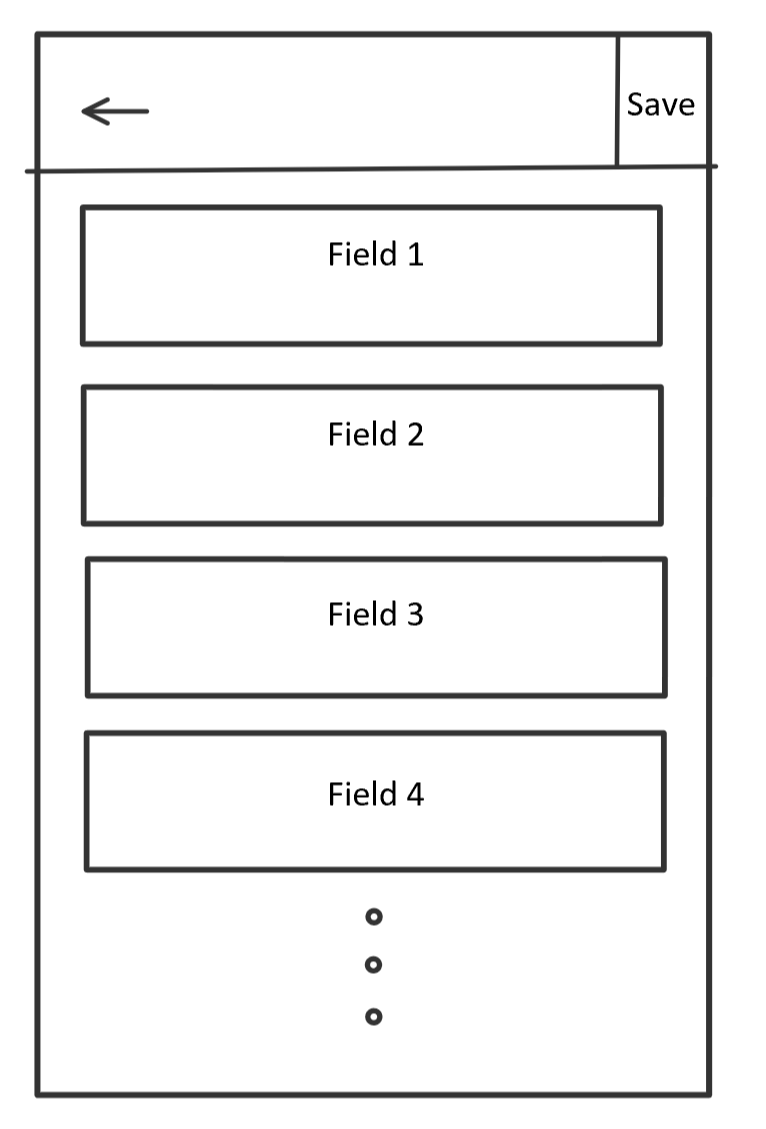
\includegraphics{eventform.PNG}
\end{center}

\section{Figure 2: Home Screen Skeleton}

The following three figures show the skeleton for the Home Screen in the three view modes: Day, Week, and Month.  Below the current date (top bar with DD/MM/YYYY) in all of the views is the Toolbar which have numbers in the boxes.  These are placeholders for the tool that will appear there.  The follow table describes what tool each number stands for:\\

\begin{center}
\begin{longtable}{ | p{0.3cm} | p{7.5cm} | }
\hline
\textbf{1} & Copy Selected Event to Clipboard \\
\hline
\textbf{2} & Paste Event on Clipboard \\
\hline
\textbf{3} & Cut Selected Event from Home to Clipboard \\
\hline
\textbf{4} & Enable Drag and Drop \\
\hline
\textbf{5} & Enable Resize \\
\hline
\textbf{6} & Create Event \\
\hline
\textbf{7} & Cycle View Mode \\
\hline
\end{longtable}
\end{center}

Additionally, in the top left corner of each of the following 3 figures, there is a button with three lines on it to represent the Hamburger menu.  When the user clicks on that, the Hamburger menu will display Figure 3a or 3b based on whether the user is logged in.

\subsection{Figure 2a: Day View}

\begin{center}
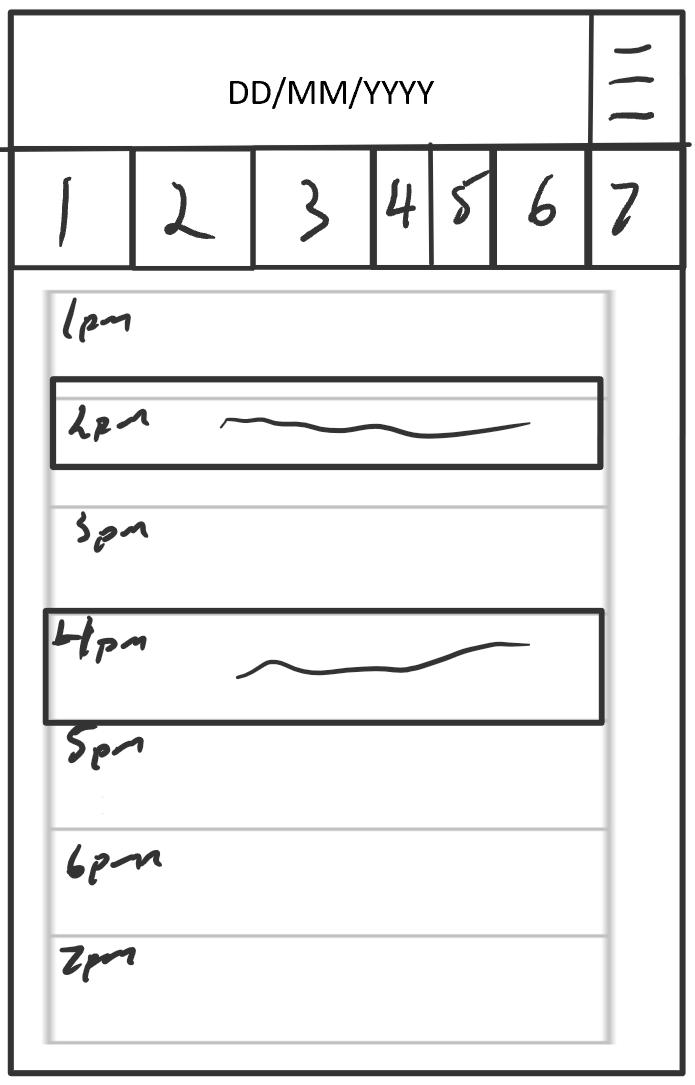
\includegraphics{day.PNG}
\end{center}

In the above figure, the calendar displays events on an hourly basis in blocks where the top and bottom represent the approximate start and end time of the event.

\subsection{Figure 2b: Week View}

\begin{center}
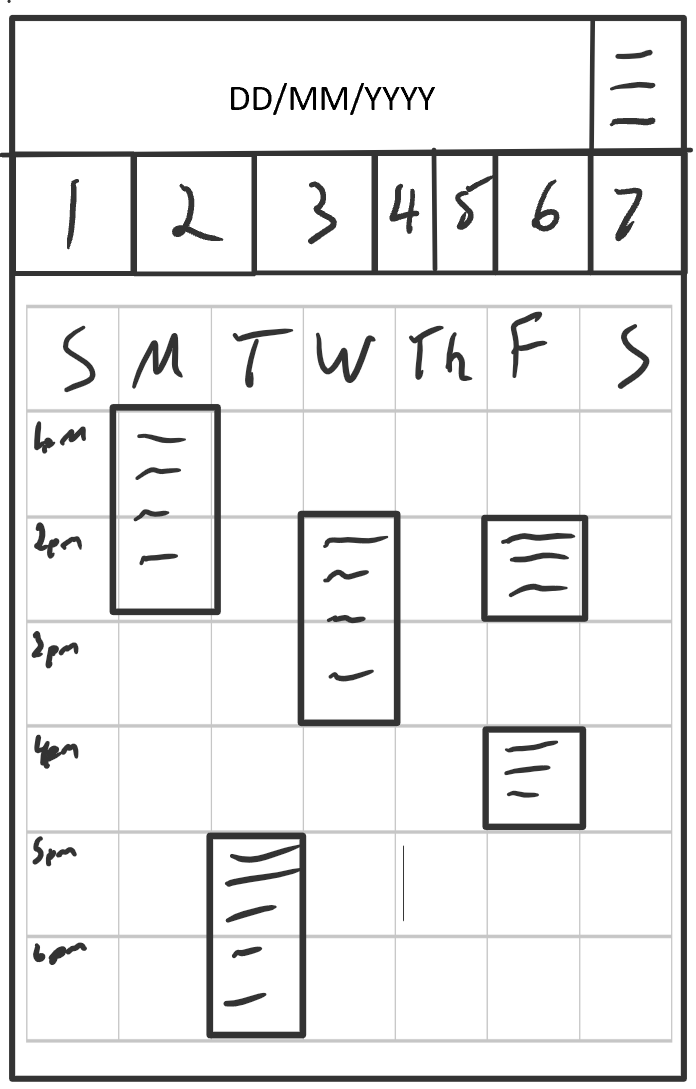
\includegraphics{week.PNG}
\end{center}

In the above figure, the calendar displays events similar to the daily view, except that it divides the horizontal width of the screen by 7 to allow all 7 days of the week to be displayed.  The top and bottom of the event boxes correspond to the approximate start and end times of the events.

\subsection{Figure 2c: Month View}

\begin{center}
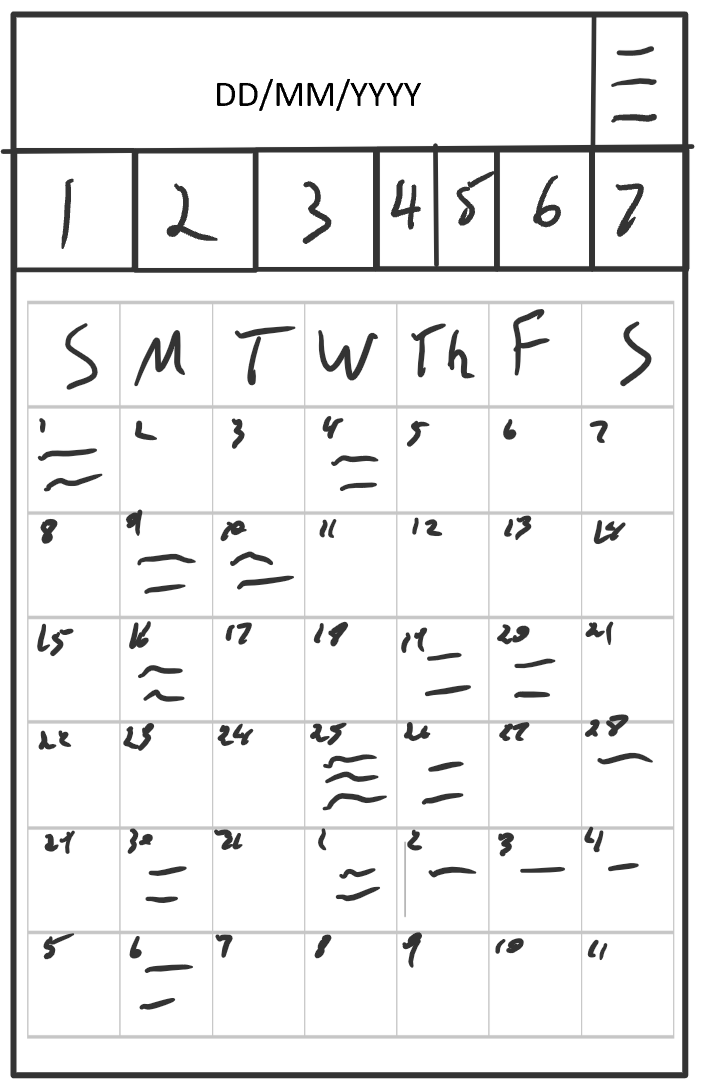
\includegraphics{month.PNG}
\end{center}


In the above figure, the calendar displays all the events in the selected month.  Each event during a particular day is listed under that day such that the user can click on it, but the separation between the events does not correspond to start and end time.  The event names are simply list and the user could click and edit them if they want to see more information.

\section{Figure 3: Hamburger Menu}

The following two figures depict the skeleton for the Hamburger Menu when the user is logged in and logged out. Each box on the Hamburger menu is a button that brings up the relevant page (except the "$<$Account Email$>$" box which just allows the user to view their email on their account).

\subsection{Figure 3a: User Logged In}

\begin{center}
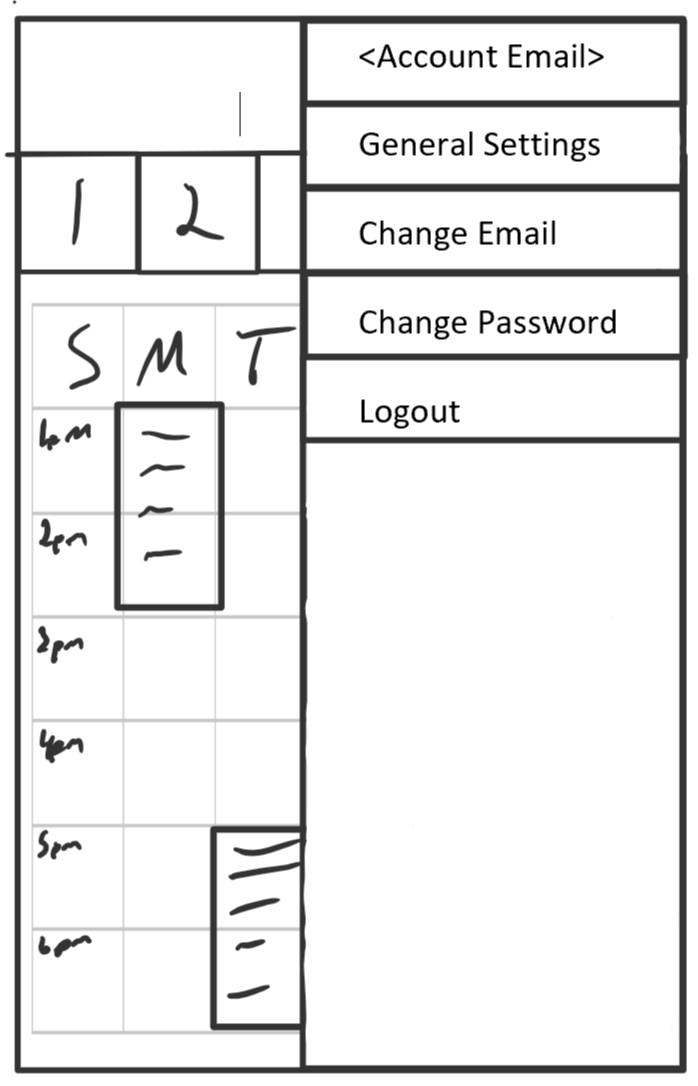
\includegraphics{hmlogin.PNG}
\end{center}

\subsection{Figure 3b: User Logged Out}

\begin{center}
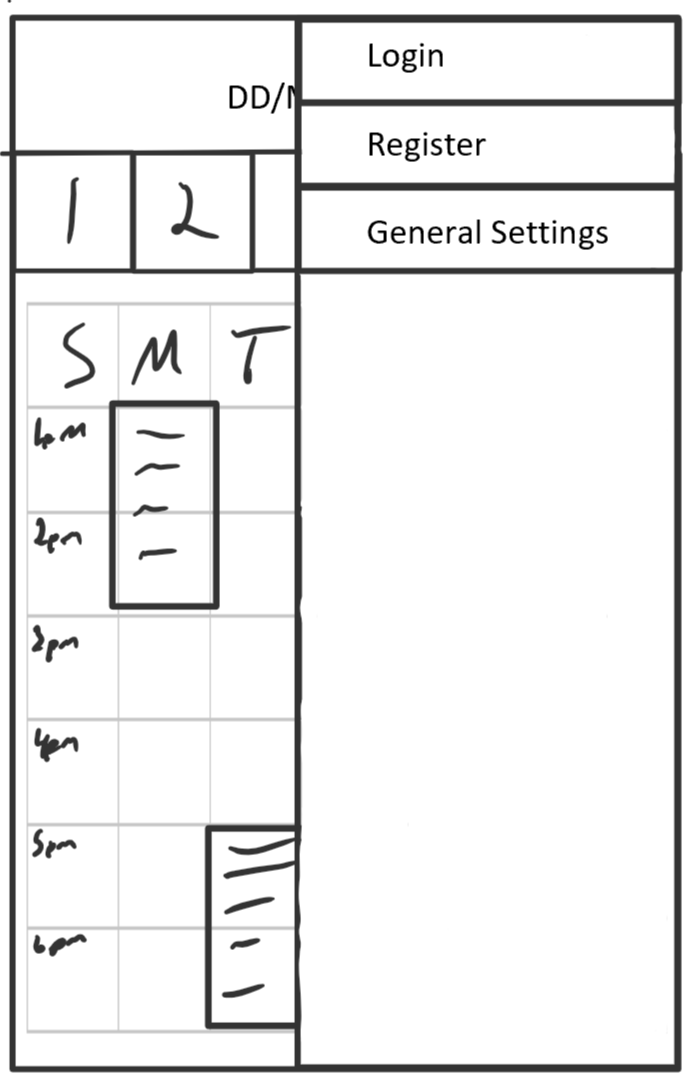
\includegraphics{hmlogout.PNG}
\end{center}

\section{Figure 4: Custom Frequency Popup}

\begin{center}
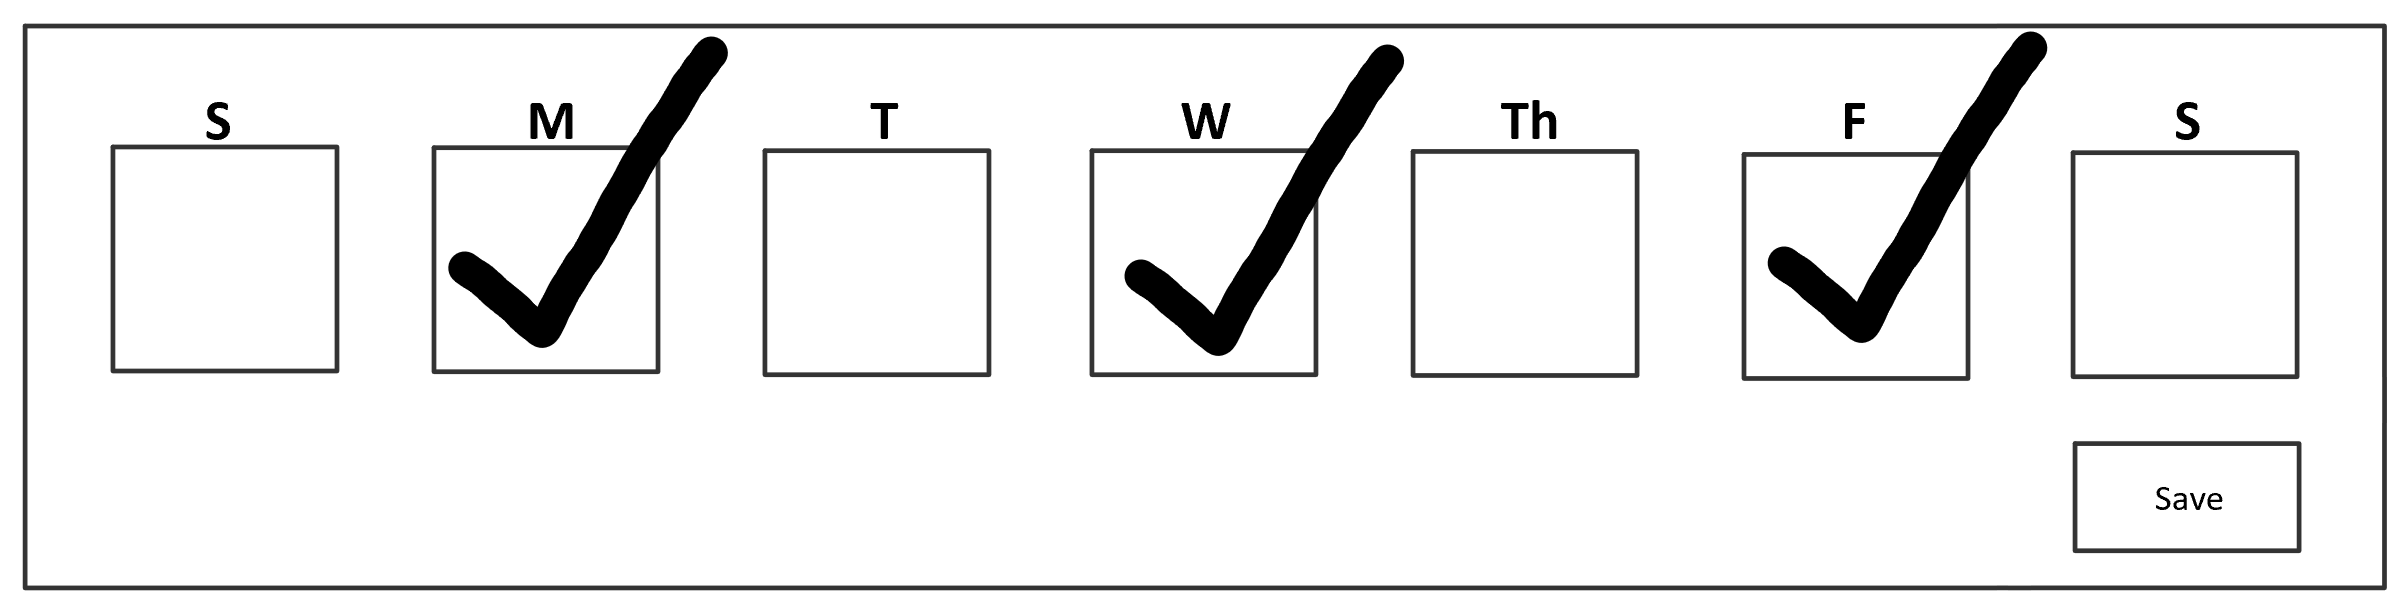
\includegraphics[width=\textwidth]{customfreq.PNG}
\end{center}

The above figure depicts the the pop-up menu skeleton that is used for creating custom frequencies.  The menu consists of 7 check boxes for each day of the week.  In the above figure, it shows a custom event that repeats every Monday, Wednesday, and Friday.
\\\\
When the user clicks "save", the options they chose are used to finish the custom Frequency setup.

\end{document}
